\label{texfile:TemplateMesh}
The next step in the model build workflow is to define a template mesh, which is a 2D finite-element mesh that is used to generate a 3D \gwf\ (and possibly a 2D \swf) finite-element mesh.   Below is an example
\footnote{This example was generated using the \tecplot\ layout file \texttt{MUT\_Examples$\backslash$6\_Abdul\_Prism\_Cell$\backslash$FIG Template Abdul.lay}. }
  showing an exploded view of a template mesh (bottom image) that was used as a basis for generating  finite-element meshs for the \gwf\ (middle image) and\swf\ (upper image) domains:
    \vspace{.2in} \\
    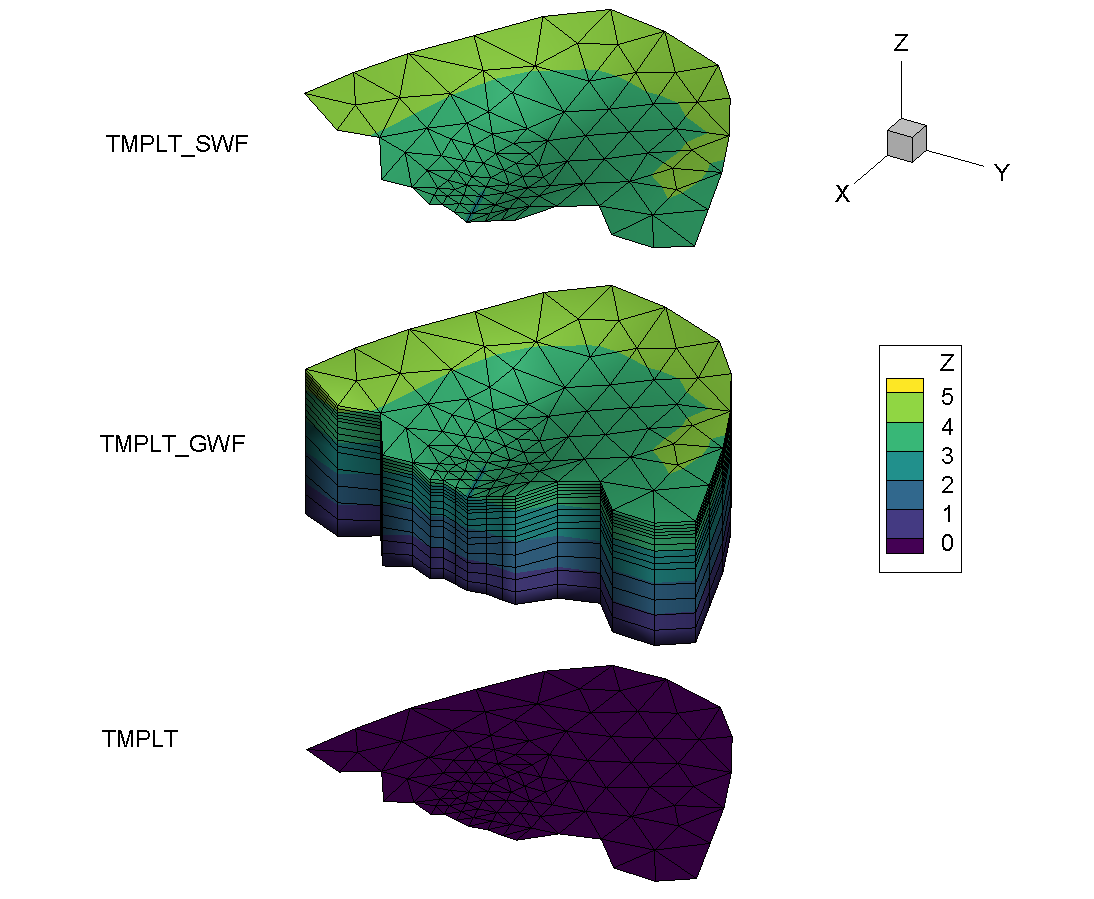
\includegraphics[width=0.87\textwidth]{tmpltAbdul}
    \vspace{.2in} \\
Some key features of this example are:
\begin{itemize}
  \item The template mesh is assigned an elevation of zero, and only the $xy$ coordinate data are used to define the other domains.
  \item The \gwf\ domain has been assigned a base elevation of zero, and a variable top elevation.
  \item The \swf\ domain has been assigned the same elevation as the \gwf\ domain i.e.\ they are coincident.
\end{itemize}

\pagebreak
 In this example, the template mesh was defined using these instructions:
 \squish
\begin{verbatim}
    2d mesh from gb
    .\gb\grid
\end{verbatim}
The instruction \textsf{2d mesh from gb}, which requires a single line of input, \texttt{.$\backslash$gb$\backslash$grid}, is documented as shown here:

\ins{2d mesh from gb}
    {
        \squish
        \begin{enumerate}
        \item \str{Prefix}  The \gb\ \footnote{\gb\ is a legacy 2D triangular finite-element grid generator.} dataset prefix, including the path to it.
        \end{enumerate}
        Given \str{Prefix}, this instruction reads the 2D finite-element grid data and uses it to define the 2D template mesh.  \str{Prefix} should contain a relative path to the dataset.  Examples of relative paths are:
        \begin{description}
        \item[.$\backslash$gb$\backslash$grid] The \mut\ input folder contains a local folder \texttt{gb} with the data set prefix \texttt{grid}.
        \item[..$\backslash$gb$\backslash$grid] The parent folder to the \mut\ input folder contains a folder \texttt{gb} with the data set prefix \texttt{grid}.
        \item[C:$\backslash$gb$\backslash$grid] Absolute path to a drive \texttt{C:} with a folder \texttt{gb} with the data set prefix \texttt{grid}.  Absolute paths are not recommended as they may lead to portability issues.
        \end{description}
        \squish
    }

To generate uniform 2D rectangular element template meshes \footnote{See for example the verification cases \texttt{MUT\_Examples$\backslash$1\_VSF\_Column} or \texttt{MUT\_Examples$\backslash$6\_Abdul\_MODHMS}} use this instruction:

\ins{generate uniform rectangles}
    {\index{generate uniform rectangles}
    \squish
    \begin{enumerate}
    \item \rnum{xl}, \inum{nbx}  Domain length and number of blocks in the $x$-direction
    \item \rnum{yl}, \inum{nby}  Domain length and number of blocks in the $y$-direction
    \end{enumerate}
    A 2D finite-element mesh composed of uniform rectangular elements will be generated. In this case, the
    grid is formed by subdividing the domain in the $x$-direction into \inum{nbx} blocks, each of length
    \textbf{\rnum{xl}/\inum{nbx}}. The domain is subdivided in a similar fashion in the $y$-direction, using the other input parameters.
    }

%This instruction reads a quadtree mesh to define a template mesh \footnote{See for example the verification case \texttt{UNDER CONSTRUCTION}}:
%
%\ins{2d quadtree mesh from groundwater vistas}
%    {\index{2d quadtree mesh from groundwater vistas}
%    \squish
%    \begin{enumerate}
%    \item \textbf{gbprefix}  The \gwv\ \footnote{\gwv\ is  third-party \mf\ development environment software.} dataset prefix, including the path to it.
%    \end{enumerate}
%    Given \textbf{gbprefix}, this instruction reads the 2D finite-element grid data and uses it to define the 2D template mesh.  The prefix should contain a relative path to the dataset.  Examples of relative paths to a Grid Builder prefix variables are:
%
%    
\includegraphics[width=.15\textwidth]{UnderConstruction}
%    }

There are two ways that \mf\ cell control volumes can be defined from the template mesh.  By default, \mut\ uses a mesh-centred approach as shown here for a triangular-element template mesh:
    \vspace{.2in} \\
    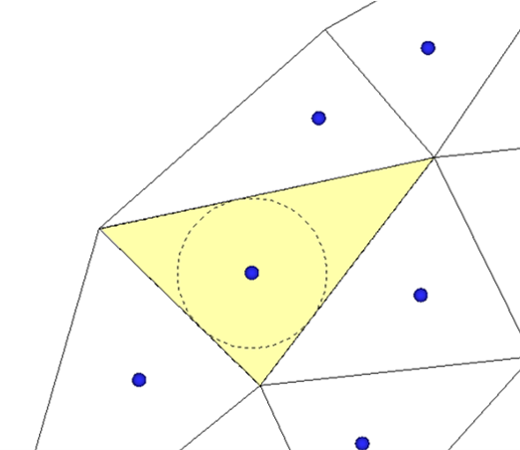
\includegraphics[width=0.6\textwidth]{MeshCentred}
    \vspace{.2in} \\
Some key features to note are:
\begin{itemize}
    \item Inner circles, which are tangent to all three element sides, are defined for each triangular element.  An example is shown by the dashed circular line in the yellow-shaded element.
    \item The blue-filled circles show the locations of the defined \mf\ cell control volumes.
    \item The vertical connection area of the cell is defined by the triangular element area (yellow-shaded triangle).
    \item The horizontal connection length of the cell is defined by the triangular element side length between neighbouring elements.
\end{itemize}

The mesh-centred approach is similar when using a  rectangular-element template mesh, with the rectangular element area and side lengths defining the vertical connection area and horizontal connection length respectively.

To use a node-centred control volume approach, add this instruction {\em before} defining any \gwf\ or \swf\ model domains:

\ins{nodal control volumes}
    {The node-centered approach will be used to define \mf\ cell centres instead of the default mesh-centered approach.
     }

The result of using a node-centred approach is shown here for a triangular-element template mesh:
    \vspace{.2in} \\
    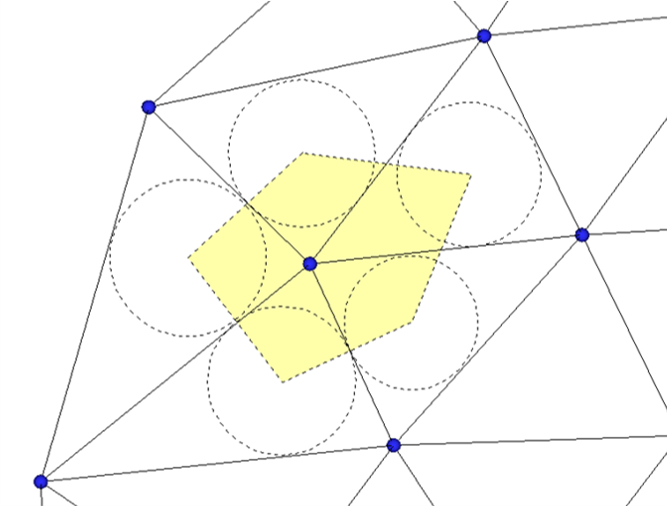
\includegraphics[width=0.6\textwidth]{NodeCentred}
    \vspace{.2in} \\
Some key features to note are:
\begin{itemize}
    \item The blue-filled circles show that the locations of the defined \mf\ cell control volumes are now located at template mesh node locations.
    \item The vertical connection area of the cell (yellow-shaded polygon) is defined by the contributing area formed by joining the inner circle centres of each element containing the template mesh node.
    \item The horizontal connection length of the cell is defined by the distance to a neghbouring node.
\end{itemize}



\includegraphics[width=.15\textwidth]{UnderConstruction} \textit{Should explain how inner circle radius is used for connection length and perpendicular area for triangles.}



